	\documentclass[10pt,oneside]{CBFT_book}
	% Algunos paquetes
	\usepackage{amssymb}
	\usepackage{amsmath}
	\usepackage{graphicx}
	\usepackage{libertine}
	\usepackage[bold-style=TeX]{unicode-math}
	\usepackage{lipsum}

	\usepackage{natbib}
	\setcitestyle{square}

	\usepackage{polyglossia}
	\setdefaultlanguage{spanish}
	



	\usepackage{CBFT.estilo} % Cargo la hoja de estilo

	% Tipografías
	% \setromanfont[Mapping=tex-text]{Linux Libertine O}
	% \setsansfont[Mapping=tex-text]{DejaVu Sans}
	% \setmonofont[Mapping=tex-text]{DejaVu Sans Mono}

	%===================================================================
	%	DOCUMENTO PROPIAMENTE DICHO
	%===================================================================

\begin{document}

% =================================================================================================
\chapter{Básicos de termodinámica}
% =================================================================================================


% =================================================================================================
\section{Energía y entropía}
% =================================================================================================

Una de las formulaciones de la 2da ley es definir la entropía. Surge de:
\[
	\frac{Q_1}{Q_2} = -\frac{T_1}{T_2} \qquad \Rightarrow \frac{Q_1}{Q_2} + \frac{T_1}{T_2} = 0 \;
	\text{reversible}
\]
\[
	\int \frac{dQ}{T} \leq 0 \qquad \text{desigualdad de Clausius}
\] 
Proceso reversible en un sistema aislado
\[
	S_{A\to B} = \int_A^B dS = 0
\]
pues 
\[
	dS =\frac{dU}{T} - \frac{p}{V}dV + \frac{\mu}{T}dN = 0
\]
pero en procesos irreversibles la variación de $S$ es cota superior:
\notamargen{La existencia de $S$ es independiente de su cálculo}
\[
	\int_A^B \frac{dQ}{T} < \int_A^B dS = S_{A\to B}.
\]

Luego, para un sistema aislado, en un proceso irreversible 
\[
	dS_I = 0 \qquad \Rightarrow \qquad \frac{dQ_I}{T} = 0
\]
y entonces
\[
	0 < \int_A^B  dS =  S_{A\to B}
\]

La entropía solo aumenta. Podría calcular $S_{A\to B}$ con un proceso reversible de $A\to B$ pero ahí 
ya tengo que intervenir sobre el sistema (no hay procesos espontáneos --en un sistema aislado-- reversibles).

En reversibles
\[
	dU = TdS - pdV + \mu dN
\]
mientras que en irreversibles
\[
	dU = ddQ_I - pdV +\mu dN, \quad \text{pero} \quad dQ_I < TdS 
\]
y entonces
\[
	dU < TdS - pdV + \mu dN
\]
% \begin{figure}[htb]
% 	\begin{center}
% 	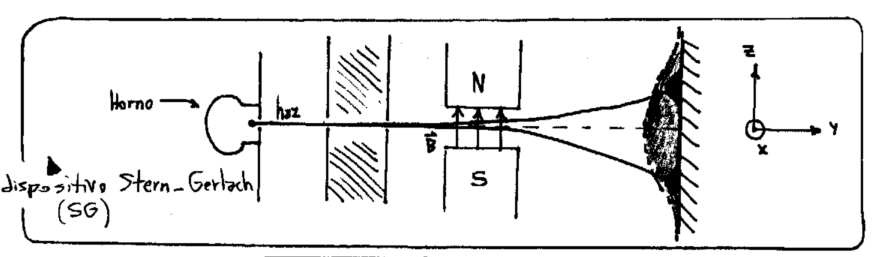
\includegraphics[width=0.8\textwidth]{images/teo2_1.pdf}	 
% 	\end{center}
% 	\caption{}
% \end{figure} 
Si $S$ es homogénea, se tiene
\[
	S = S(\lambda U, \lambda X, \{\lambda N_i\}) = \lambda S( U, X, \{ N_i\})
\]
y además si \notamargen{En un sistema $PVT$ $Y=-p$.}
\[
	TdS = dU - YdX - \mu_i dN_i
\]
\[
	\dtot{S}{\lambda} = S = \dpar{S}{\lambda U}\dtot{\lambda U}{\lambda} +
	\dpar{S}{\lambda X}\dtot{\lambda X}{\lambda} +
	\dpar{S}{\lambda N_i}\dtot{\lambda N_i}{\lambda}
\]
\[
	S = \dpar{S}{\lambda U} U + \dpar{S}{\lambda X} X + \dpar{S}{\lambda N_i} N_i
\]
\[
	\dpar{}{\lambda U}\left[ S(\lambda U)\right] = 
	\dpar{}{\lambda U}\left[ \lambda S( U)\right] = \dpar{S}{U} = \frac{1}{T}
\]
y procediendo del mismo modo con $Y,\mu$
\[
	S = \frac{1}{T} U + \frac{-Y}{T} X + \frac{-\mu_i}{T} N_i
\]
y arribamos a la ecuación fundamental
\[
	TS = U - YX - \mu_i N_i 
\]
o bien
\[
	U = TS + YX + \sum_i \mu_i N_i
\]

La primera ley (en sistemas reversibles) era 
\[
	dU = TdS + YdX + \sum_i \mu_i dN_i
\]
y a $S,V,N$ constantes 
\[
	dU^R = 0 \qquad dU^I \leq 0
\]
la mínima $U$ es equilibrio.
Si existe trabajo que no es de volumen resulta 
\[
	dU < -dW_\text{libre}
\]
\[
	\frac{dQ}{dT} = \frac{dU}{T} + \frac{p}{T}dV - \frac{\mu}{T}dN = \frac{dQ}{dT} \leq dS
\]

Si el sistema está aislado será
\[
	0 \leq dS \quad \text{condición de equilibrio}
\]
alcanzando el máximo ya no puede disminuir la entropía.


% =================================================================================================
\section{Transformadas de Legendre de las funciones termodinámicas}
% =================================================================================================

\[
	f(x,y,z) \qquad \text{con pendientes} \quad \dpar{f}{x},\dpar{f}{y},\dpar{f}{z}
\]
entonces 
\[
	\varphi(f_x,y,z) = f(x,y,z) - \left. x \dpar{f(x,y,z)}{x}\right|_{y,z}
\]
es la transformada de Legendre respecto de $x$, mientras que 
\[
	\varphi(f_x,f_y,z) = f(x,y,z) - x \dpar{f}{x} - y \dpar{f}{y}
\]
es la transformada de Legendre respecto de $y$.

La transformada de Legendre transforma una función homogénea en otra función homogénea, mantiene el
carácter de función de estado.
\[
	d\varphi(f_x,y,z) = df - dx \dpar{f}{x} - x d\left( \dpar{f}{y} \right)
\]

Para el caso de la energía
\[
	U=U(S,V,N) \qquad \qquad dU = TdS - pdV + \mu dN
\]
y entonces
\[
	A = U - \left. S\dpar{U}{S}\right|_{V,N} = U - ST \qquad \Rightarrow \qquad  A=A(T,V,N)
\]
\[
	H = U - \left. V\dpar{U}{V}\right|_{S,N} = U + pV \qquad \Rightarrow \qquad  H=H(S,p,N)
\]
\[
	G = U - \left. S\dpar{U}{S}\right|_{V,N} - \left. V\dpar{U}{V}\right|_{S,N} = 
	U - ST + pV \qquad \Rightarrow \qquad  G=G(T,p,N)
\]
\[
	dA = dU - SdT - TdS = -SdT - pdV + \mu dN
\]
\[
	dA \leq -SdT - pdV + \mu dN 
\]
entonces $A$ mínimo es equilibrio a $T,V,N$ constantes.

La idea de las transformadasd de Legendre es pasar la dependencia de cierto juego de variables a otro
que podría ser más apropiado par el sistema en cuestión.

Sistema aislado en equilibrio, entonces se tendrá $S$ máxima y como $S(U,V,N)$ y considero fluctuación
energética
\[
	\left. \dpar{S}{U} \right|_{\text{eq}} = 0 \qquad \left. \dpar2{S}{U} \right|_{\text{eq}} < 0
\]
\[
	\delta S_{\mathrm{orden 2}} = \frac{1}{2} \left. \dpar2{S}{U} \right|_{\text{eq}} \delta U^2
\]

% =================================================================================================
\section{Gas de Van der Waals}
% =================================================================================================

Van der Waals incorpora la interacción molecular. \notamargen{Esta subsección tiene cinco gráficos}
\[
	\left( p +\frac{an^2}{V^2} \right)(V- nb) = nRT
\]
donde $a,b(T)$ caracterizan al gas en cuestión.

La función $p=p(V)$ tiene tres extremos para $T<T_c$,
\[
	\dpar{p}{V} = 0
\]
En $T=T_c$ es
\[
	\left.\dpar{p}{V} \right|_{T_c} = 0 \qquad \left.\dpar[2]{p}{V} \right|_{T_c} = 0
\]
punto de inflexión
\[
	v_c = 3b \qquad p_c = \frac{a}{27b^2} \qquad T_c = \frac{8a}{27Rb}
\]
y eso lleva a la ley de estados correspondientes
\[
	\left( \bar{p} + \frac{3}{\bar{v}^2} \right)(3 \bar{v} - 1)= 8\bar{T}
\]

De Van der Waals al virial
\[
	p = \frac{nRT}{(V-nb)} - a \left(\frac{n}{V} \right)^2 = 
	\frac{nRT}{V(1-b/v)}- \frac{a}{v^2}
\]
\[
	p = \frac{RT}{v}\left[ 1 + \frac{b}{v} - \frac{a}{vRT} \right] =
	p = \frac{RT}{v}\left[ 1 + \frac{1}{v}\left( b - \frac{a}{RT} \right) \right]
\]
y el último paréntesis es el primer coeficiente del virial.

Un potencial intermolecular está compuesto de una zona repulsiva (carozo duro) y una atractiva (cola)
\[
	V_{eff} = V-b \qquad (\mathrm{menor volumen por el carozo})
\]
\[
	p = \frac{RT}{V-b} - \left(\frac{a}{V}\right)^2 \qquad (\mathrm{menor presión por la atractividad})
\]
y entonces, por mol de sustancia,
\[
	\left( p +\frac{a^2}{V^2} \right)(V- b)= RT
\]

$b$ corrige el volumen que es ahora menor porque las partículas ocupan espacio. $a$ corrige la presión dado que la 
atracción tiende a formar pares bajando la presión sobre las paredes.

Las funciones respuesta tienen signo errado dentro de la zona del rulo\notamargen{Recordemos que
\[ -\frac{1}{v}\dpar{v}{p}=\kappa_T > 0\]}
\[
	\dpar{p}{V}>0 \rightarrow  \dpar{v}{p} >0 \Rightarrow \kappa_T < 0 \qquad (\mathrm{MAL})
\]
\[
	dT = -SdT + VdP + \mu dN
\]
dada la isoterma y que $N$ es constante 
\[
	dG = Vdp \rightarrow dg = v dP \quad (\mathrm{molar})
\]
$G$ es cóncava en $p$ entonces 
\[
	v = \left.\dpar{g}{p} \right|_{T,N}, \qquad  
	\dpar{v}{p} =\left.\dpar[2]{g}{p} \right|_{T,N} < 0
\]
y luego 
\[
	\Delta g = \int_{p_c}^{p_G} v dp = 0
\]
entonces 
\[
	\int_C^D + \int_D^E + \int_E^F + \int_F^G = 0
\]
y si se invierten puntos para tener un recorrido según las flechas se llega a 
\[
	\int_C^D - \int_E^D = \int_F^E - \int_F^G 
\]

Áreas inguales determinan entonces los puntos C y G de forma que se corrige Van Der Waals para dar curvaturas
correctas. En la región de coexistencia hemos trocado
\[
	\dpar{p}{V} > 0 \quad \mathrm{por} \quad \dpar{p}{V}=0
\]
lo cual da $\kappa_T \to \infty$ en lugar del $\kappa_T < 0$ (que es incorrecto).









% \bibliographystyle{CBFT-apa-good}	% (uses file "apa-good.bst")
% \bibliography{CBFT.Referencias} % La base de datos bibliográfica

\end{document}
